%% This is file `jasr-template.tex',
%% 
%% Copyright 2019-2020 Elsevier Ltd
%% 
%% This file is part of the 'Elsarticle Bundle'.
%% ---------------------------------------------
%% 
%% It may be distributed under the conditions of the LaTeX Project Public
%% License, either version 1.2 of this license or (at your option) any
%% later version.  The latest version of this license is in
%%    http://www.latex-project.org/lppl.txt
%% and version 1.2 or later is part of all distributions of LaTeX
%% version 1999/12/01 or later.
%% 
%% The list of all files belonging to the 'Elsarticle Bundle' is
%% given in the file `manifest.txt'.
%% 
%% Template article for Elsevier's document class `elsarticle'
%% with harvard style bibliographic references
%%
%% $Id: jasr-template.tex 188 2020-11-16 05:18:23Z rishi $
%%
%% Use the option review to obtain double line spacing
%\documentclass[times,review,preprint,authoryear]{elsarticle}

%% Use the options `twocolumn,final' to obtain the final layout
%% Use longtitle option to break abstract to multiple pages if overfull.
%% For Review pdf (With double line spacing)
%\documentclass[times,twocolumn,review]{elsarticle}
%% For abstracts longer than one page.
%\documentclass[times,twocolumn,review,longtitle]{elsarticle}
%% For Review pdf without preprint line
%\documentclass[times,twocolumn,review,nopreprintline]{elsarticle}
%% Final pdf
\documentclass[times,twocolumn,final,authoryear]{elsarticle}
%%
%\documentclass[times,twocolumn,final,longtitle]{elsarticle}
%%

%%
%% Stylefile to load JASR template
\usepackage{jasr}
\usepackage{framed,multirow}

%% The amssymb package provides various useful mathematical symbols
\usepackage{amssymb}
\usepackage{latexsym}

%% For line numbers
%\usepackage[switch]{lineno}

% Following three lines are needed for this document.
% If you are not loading colors or url, then these are
% not required.
\usepackage{url}
\usepackage{xcolor}
\usepackage{multirow}
%\usepackage{tablefootnote}
\definecolor{newcolor}{rgb}{.8,.349,.1}

\usepackage[citebordercolor=white]{hyperref}
\usepackage{rotating}
\usepackage{aas_macros}
\usepackage{pdflscape}
\usepackage{longtable}
\usepackage{amssymb,amsmath,amsthm}
\usepackage{siunitx}
\usepackage[utf8]{inputenc}
\usepackage{etoolbox}
\usepackage{fixltx2e}
\journal{Advances in Space Research}

\begin{document}

\verso{Tarango-Yong \textit{et. al}}

\begin{frontmatter}

\title{Ionospheric Disturbances in Mexican Territory Produced by Objects Entering the Atmosphere from Space \tnoteref{tnote1}}%
%\tnotetext[tnote1]{This is an example for title footnote coding.}

\author[1]{Jorge \snm{Tarango-Yong}\corref{cor1}}
\cortext[cor1]{Tel.: +52-443-476-5525;  \\
  email: jorge.tarango@comunidad.unam.mx
}

\author[1]{Mario \snm{Rodriguez-Martinez}\corref{cor2}}
\cortext[cor2]{email: m.rodriguez@enesmorelia.unam.mx}
%\fntext[fn1]{This is author footnote for second author.}
\author[1]{Raul \snm{Guti\'errez-Zalapa}\fnref{fn1}}
%% Third author's email
%\ead{author3@author.com}
%\author[2]{Given-name4 \snm{Surname4}}

\address[1]{Escuela Nacional de Estudios Superiores, UNAM, campus Morelia, Antigua Carretera a P\'atzcuaro No. 8701
Col. Ex Hacienda de San Jos\'e de la Huerta, Morelia, Michoac\'an, 58190, M\'exico}
%\address[2]{}

\received{1 May 2013}
\finalform{10 May 2013}
\accepted{13 May 2013}
\availableonline{15 May 2013}
\communicated{S. Sarkar}


\begin{abstract}
%%%
Please type your abstract here, and the rest of the text, figures,
tables, equations etc. in the main body. Please do not modify LaTeX\ 
commands unless you need to modify them and know how to do it.
%%%%
\end{abstract}

\begin{keyword}
%% MSC codes here, in the form: \MSC code \sep code
%% or \MSC[2008] code \sep code (2000 is the default)
%\MSC 41A05\sep 41A10\sep 65D05\sep 65D17
%% Keywords
\KWD Space Sciences\sep Atmosphere%\sep Keyword3
\end{keyword}

\end{frontmatter}

%% For linenumbers
%\linenumbers

%% main text
\section{Introduction}
\label{sec1}
The Earth's magnetic field represents a final obstacle to the Solar Wind (SW) flux. When descelerated and defected by a non colisional shock wave in the flux direction, generates a cavity known as magnetosphere \citep{Blanco-Cano:2004}. Since the Earth is embedded in this SW flux, is known that under adequated physical conditions (e.g magnetic reconnection) may exist some coupling between the magnetosphere and the Earth's ionosphere \citep{Zolesi:2014, Cnossen:2014}.

The Sun plays an important role in the physical proccesses that occur in the terrestrial magnetosphere-ionosphere system. When the SW interacts with the Earth's magnetosphere, particles may permeate the internal region via magnetic reconnection and penetrate to polar zones and generate boreal or austral auroras thus altering the system \citep{Vazquez:2016, Oka:2011}. By the other hand, the Extreme Ultraviolet Radiation (EUV) and X-rays coming from the Sun may interact with the neutral atmoshere via photoionization \citep{Vlasov:2010}. However, in both cases the final result is that the ionosphere's free electrons population is altered.

Some Ionospheric Perturbations (IP) become relevant due to their spatial and temporal scale in the Space Weather scenario. At intermediate latitudes, the most common in the ionosphere are known as Traveling Ionospheric Disturbances (TIDs). Typically they divide into two groups: a) large scale TIDs, associated with geomagnetic storms with sizes of \SI{\sim 2000}{km}, periods of \SI{\sim 1}{h} and velocities of \SI{\sim 700}{km.s^{-1}}, and b) Medium-scale TIDs, which are not fully associated with geomagnetic storms, present sizes of \SI{\sim 100}{km}, periods from 10 minutes to 1 hour and velocities between \SI{50}{km.s^{-1}} and \SI{1e2}{km.s^{-1}} \citep{Helmboldt:2012}. Diverse methods have benn used to study TIDs, such as incoherent dispersion radars, high frequency Doppler emmisors, data from Global Positioning System (GPS) stations or even radiotelescopes like the VLA or the Mexican Array Radio Telescope (MEXART) \citep{Chilcote:2015, Rodriguez:2014}.

On the other side, the Earth's ionosphere may be affected or modified by other proccesses, particularly there are studies that show how the Vetical Total Electron Content (vTEC) due to shock waves generated for rockets launched to space \citep{Lin:2014}. Similar proccesses modify the Earth's ionosphere due to objects entering the athmosphere from space, such as meteoroids like the one which fell on Chelyabinsk at 2013 \citep{Yang:2014}. Previously, the ionospheric perturbations produced by this object were studied using two independent methods: a) detecting vTEC pertubations using GPS station near the impact location. And b) a wavelets analysis for detection of ...

In 2020 a meteoroid passed in mexican territory through mexican territory, which also was studied \citep{Sergeeva:2020}. The meteoroid was recorded with outdoor cameras in different locations. The trajectory could be estimated, as well as other physical parameters.

In this work we will show a similar analysis for a sample of meteoroids detected in mexican territory by different methods. The first subsample consists in objects detected by the Geostationary Lightning Mapper (GLM) whose sizes are estimated between a few decimeters to meters in diameter \citep{GOODMAN:2013, Jenniskens:2018, Rumpf:2019}. The second subsample will consist in objects detected by ocular witnesses from the American Meteor Society and as comparisson we will include the morelian meteoroid reported in \citet{Sergeeva:2020} and the Chelyabinsk event \citet{Yang:2014}. The paper is arranged in the following way: \S \ref{sec:methodology} describes the samples of meteoroids as well of the properties that can be obtained from direct observations. Also describes the GPS data corresponding to the dates and locations where each object was located. \S \ref{sec:bolides} shows physical parameters of meteoroids obtained from the observed heights and energies. Finally, section \S \ref{sec:vTEC-maps} shows the vTEC maps and scintillation indices obtained from GPS observations.  
%Please use \verb+elsarticle.cls+ for typesetting your paper. Additionally,
%make sure not to remove the package \verb+jasr.sty+ already included in the
%preamble:
%\begin{verbatim} 
%  \usepackage{jasr}
%\end{verbatim}

%Make sure to have the file \verb+model5-names.bst+ to produce the references in
%the correct format. 

%Any instructions relevant to the \verb+elsarticle.cls+ are
%applicable here as well. See the online instruction available at:
%\makeatletter
%\if@twocolumn
%\begin{verbatim}
% https://support.stmdocs.in/wiki/
% index.php?title=Elsarticle.cls
%\end{verbatim}
%\else
%\begin{verbatim}
% https://support.stmdocs.in/wiki/index.php?title=Elsarticle.cls
% \end{verbatim}
%\fi
%\makeatother

%Following commands are defined for this journal which are not in
%\verb+elsarticle.cls+. 
%\begin{verbatim}
%  \received{}
%  \finalform{}
%  \accepted{}
%  \availableonline{}
%  \communicated{}
%\end{verbatim}


%\subsection{Subsection}
%This is only a \LaTeX\ template if you need one. 
%See the detailed guidelines for manuscript preparation 
%and submission at:
%\begin{verbatim}
%https://ees.elsevier.com/asr
%\end{verbatim}


\section{Observational data}
\label{sec:methodology}
\subsection{Meteors Databases}
\label{ssec:databases}
We selected a sample of meteors which were observed in mexican territory from the Geostationary Lightning Mapper \citep{GOODMAN:2013}. Orignally this project was designed to detect ligthning activity in earth's athmosphere, but has been proven that also can detect bolides entering the athmosphere. The detection comes from two satellites called GOES-16 and GOES-17 orbiting the earth in geostationary orbits. %Figure  shows the area where GOES-16 and GOES-17 detect activity on a lightning flash rate map; in mexican territory clearly both satellites can make detections. %Create a figure where the area coverage of GOES-16 and GOES-17 is shown.
We used the interactive database available at \url{https://neo-bolide.ndc.nasa.gov/#/}. These data are publicly available and easily downloaded from the same website. For each event we can obtain the recorded trajectory of meteors and the corresponding light curve. THe GLM satellites have an umbral magnitude for detection of -14. At this magnitude, a meteor is considered a bolide, and is expected to be at least decimeter-sized (in diameter) to reach such brightness. In the other hand, too bright meteors will saturate the detectors, and thus, lowering the quality of data. The result of this factors implies that the range in size of the objects in our sample varies in diameter between decimeter to meter size. %The sample was chosen following the next criteria:%selected in such way we chose the most probable objects to be detected by GPS sources in mexican territory and its surroundings: 
Each event also has assigned a confidence ratio, from low confidence to high, depending in how bright is the event itself and if the trajectory recorded by GLM ressembles (or not) a straight line. We chose only events whose confidence ratio is high, in oreder to be sure we chose the brightest objects, and thus, in the diameter size of bolides, we favored the meter-sized ones. In table \ref{tab:table-meteors} we list the object we chose to do this work, order in chronological order. The columns of the table, from left to right are and ID to enumerate the meteors in the sample, the date and time each meteor was detected, the duration of the detection, their respective coordinates and the estimated height of the meteor over the ground at the time of the detection. GOES-16 and GOES-17 systematically detect the meteors at slightly different positions and at slightly different times, so we calculated the mean of the duration, latitude and longitude reported by both satellites for each event, and used the standard deviation as the uncertainties.

From table \ref{tab:table-meteors} is also clear that the duration of all the bolides detection last less than a second. This obsevation suggests that the bolides remain undetected by the GLM satellites until they get fragmented due to stagnation presure when they release a huge amount of energy and thus they become detectable.


%From the light curves we can estimate the total radiated energy and then convert it to the total kinetic energy through a relation. With this energy we may estimate physical parameters with the cloud fragmentation model form wheeler et al.

%\begin{itemize}
%    \item The objects were detected inside mexican territory and its surroundings.
%    \item The objects were detected by both satellites GOES 16 and GOES 17 (stereo)
%    \item The detection has been assigned a high confidence ratio.
%\end{itemize}



\begin{table*}
  \centering
  \footnotesize
  \caption{List of bolides detected in mexican territory (plus one detected near Venezuela and one detected near Cuba), detected by the Geostationary Lighning mapper. The events are listed in chronological order. The listed duration, latitude and longitude correspond to the mean of the measurements of both GOES satellites. The uncertainties correspond to the respecting mean deviation.}
\label{tab:table-meteors}
\begin{tabular}{rrrrrrrrrr}
\hline
ID & Date of event  & Start Time (UT)  & Duration (seconds) & Latitude (deg) & Longitude (deg)& Altitude (km) & Energy (kT )\\\hline
GLM-00 & 2019-02-01 & 18:17:09 & $2.651\pm 0.4907$ & $22.45 \pm 0.071$ & $-83.50  \pm  0.424$ & 24           & 2.0978196 +/- 0.42361329      \\         
GLM-01 & 2019-05-23 & 16:36:18 & $0.197\pm 0.0000$ & $24.30 \pm 0.000$ & $-101.60 \pm  0.849$ & 28           & 0.011954659 +/- 7.4054404e-3  \\
GLM-02 & 2019-07-18 & 14:30:30 & $0.058\pm 0.0000$ & $27.20 \pm 0.000$ & $-103.15 \pm  0.778$ & 72           & 5.7827709e-3 +/- 3.9334336e-3 \\
GLM-03 & 2019-08-10 & 11:18:48 & $0.199\pm 0.0757$ & $21.50 \pm 0.000$ & $-102.50  \pm 0.849$ & 92           & 0.010556123 +/- 6.6488245e-3  \\
GLM-04 & 2019-10-03 & 07:55:33 & $0.106\pm 0.0297$ & $25.65 \pm 0.071$ & $-96.25 \pm   0.778$ & 74           & 2.9915536e-3 +/- 2.2000998e-3 \\
GLM-05 & 2019-10-09 & 06:08:11 & $0.103\pm 0.0078$ & $23.60 \pm 0.000$ & $-111.95 \pm  0.212$ & 32           & 0.021837042 +/- 0.012429732   \\
GLM-06 & 2019-11-16 & 09:36:04 & $0.396\pm 0.0134$ & $20.30 \pm 0.000$ & $-100.55 \pm  0.919$ & 82           & 7.5423706e-3 +/- 4.9626060e-3 \\
GLM-07 & 2019-11-17 & 15:36:01 & $0.116\pm 0.0035$ & $31.70 \pm 0.000$ & $-117.70 \pm  1.131$ & 88           & 0.022397444 +/- 0.012701445   \\
GLM-08 & 2019-11-19 & 07:57:40 & $0.097\pm 0.1138$ & $20.00 \pm 0.000$ & $-88.40 \pm   1.131$ & 99           & 1.5012507e-3 +/- 1.1909667e-3 \\
GLM-09 & 2019-11-26 & 13:23:20 & $0.078\pm 0.0290$ & $23.90 \pm 0.000$ & $-108.70 \pm  0.849$ & 81           & 4.9551290e-3 +/- 3.4345742e-3 \\
GLM-10 & 2019-12-04 & 09:42:54 & $0.173\pm 0.0028$ & $31.50 \pm 0.000$ & $-113.65 \pm  0.919$ & 77           & 0.029149047 +/- 0.015891049   \\
GLM-11 & 2019-12-15 & 14:50:49 & $0.127\pm 0.0134$ & $27.70 \pm 0.000$ & $-114.10 \pm  0.849$ & 78           & 0.010556123 +/- 6.6488245e-3  \\
GLM-12 & 2019-12-29 & 16:16:35 & $0.062\pm 0.0134$ & $29.60 \pm 0.000$ & $-116.35 \pm  0.919$ & 79           & 4.2084911e-3 +/- 2.9746446e-3 \\
GLM-13 & 2020-01-03 & 14:10:17 & $0.113\pm 0.0085$ & $30.20 \pm 0.000$ & $-117.65 \pm  0.919$ & 74           & 0.011607116 +/- 7.2187549e-3  \\
GLM-14 & 2020-01-06 & 16:39:27 & $0.118\pm 0.0042$ & $31.40 \pm 0.000$ & $-108.20 \pm  0.990$ & 81           & 0.015448801 +/- 9.2392402e-3  \\
GLM-15 & 2020-01-15 & 15:00:33 & $0.213\pm 0.1351$ & $19.45 \pm 0.071$ & $-95.55 \pm   0.919$ & 93           & 0.012559739 +/- 7.7284725e-3  \\
GLM-16 & 2020-02-12 & 09:25:40 & $0.210\pm 0.0226$ & $18.90 \pm 0.000$ & $-93.50 \pm   0.849$ & 90           & 8.2107211e-3 +/- 5.3440405e-3 \\
GLM-17 & 2020-03-03 & 12:33:27 & $0.062\pm 0.0007$ & $18.25 \pm 0.071$ & $-106.35 \pm  0.636$ & 77           & 3.4441157e-3 +/- 2.4922397e-3 \\
GLM-18 & 2020-03-31 & 19:31:52 & $0.105\pm 0.0573$ & $28.45 \pm 0.071$ & $-112.05 \pm  0.636$ & 61           & 7.2469897e-3 +/- 4.7924800e-3 \\
GLM-19 & 2020-04-08 & 16:25:28 & $0.120\pm 0.0926$ & $26.10 \pm 0.000$ & $-93.90 \pm   0.849$ & 78           & 4.0292119e-3 +/- 2.8626279e-3 \\
GLM-20 & 2020-04-18 & 17:43:25 & $0.139\pm 0.0106$ & $29.00 \pm 0.000$ & $-106.55 \pm  0.919$ & 82           & 5.8303967e-3 +/- 3.9618242e-3 \\
GLM-21 & 2020-04-20 & 16:05:22 & $0.318\pm 0.1655$ & $28.15 \pm 0.071$ & $-97.85 \pm   1.061$ & 88           & 0.031378060 +/- 0.016913982   \\
GLM-22 & 2020-04-25 & 11:03:09 & $0.323\pm 0.0813$ & $32.15 \pm 0.071$ & $-111.60 \pm  1.131$ & 84           & 0.021997346 +/- 0.012507576   \\
GLM-23 & 2020-04-28 & 19:31:52 & $0.105\pm 0.0573$ & $28.45 \pm 0.071$ & $-112.05 \pm  0.636$ & 29           & 0.12687833 +/- 0.053736010    \\
GLM-24 & 2020-05-08 & 10:06:16 & $0.490\pm 0.0750$ & $21.60 \pm 0.000$ & $-92.40 \pm   0.849$ & 81           & 0.033207253 +/- 0.017743607   \\
GLM-25 & 2020-07-15 & 19:58:28 & $0.693\pm 0.0495$ & $24.00 \pm 0.000$ & $-108.35 \pm  0.495$ & 53           & 0.020548979 +/- 0.011800641   \\
GLM-26 & 2020-08-07 & 13:29:57 & $0.163\pm 0.0057$ & $28.80 \pm 0.000$ & $-106.05 \pm  0.919$ & 89           & 0.014606987 +/- 8.8040841e-3  \\
GLM-27 & 2020-09-13 & 16:41:59 & $0.184\pm 0.0078$ & $28.45 \pm 0.071$ & $-113.75 \pm  0.919$ & 85           & 0.010995616 +/- 6.8881646e-3  \\
GLM-28 & 2020-09-30 & 12:28:11 & $0.100\pm 0.0078$ & $24.90 \pm 0.000$ & $-110.90 \pm  0.849$ & 83           & 0.014013965 +/- 8.4951275e-3  \\
GLM-29 & 2020-11-16 & 12:28:11 & $0.100\pm 0.0078$ & $24.90 \pm 0.000$ & $-110.90 \pm  0.849$ &106           & 0.052044572 +/- 0.025868548   \\
GLM-30 & 2020-11-17 & 12:53:41 & $0.404\pm 0.0262$ & $23.00 \pm 0.000$ & $-102.45 \pm  0.919$ & 93           & 0.060624247 +/- 0.029367156   \\
GLM-31 & 2020-12-19 & 10:18:14 & $0.407\pm 0.0110$ & $21.95 \pm 0.071$ & $-101.60 \pm  0.990$ & 98           & 0.060272985 +/- 0.029225978   \\
GLM-32 & 2020-12-23 & 09:43:01 & $0.148\pm 0.0014$ & $25.75 \pm 0.071$ & $-111.25 \pm  0.778$ & 81           & 0.012127937 +/- 7.4982028e-3  \\
GLM-33 & 2020-12-29 & 15:20:54 & $0.118\pm 0.0014$ & $16.80 \pm 0.000$ & $-102.20 \pm  0.707$ & 81           & 0.013161054 +/- 8.0470909e-3  \\
GLM-34 & 2021-03-31 & 09:01:17 & $0.753\pm 0.3083$ & $20.15 \pm 0.071$ & $-92.95 \pm  0.212$  & 24           & 0.054259119 +/- 0.026782008   \\
GLM-Ven& 2019-06-22 & 21:25:45 & $4.873\pm 0.0000$ & $14.9 \pm 0.000$  & $-65.8 \pm 0.000$    & 25           & 6.1014359 +/- 0.81239700      \\ \hline
\end{tabular}
\end{table*}

\begin{figure}
  \centering
  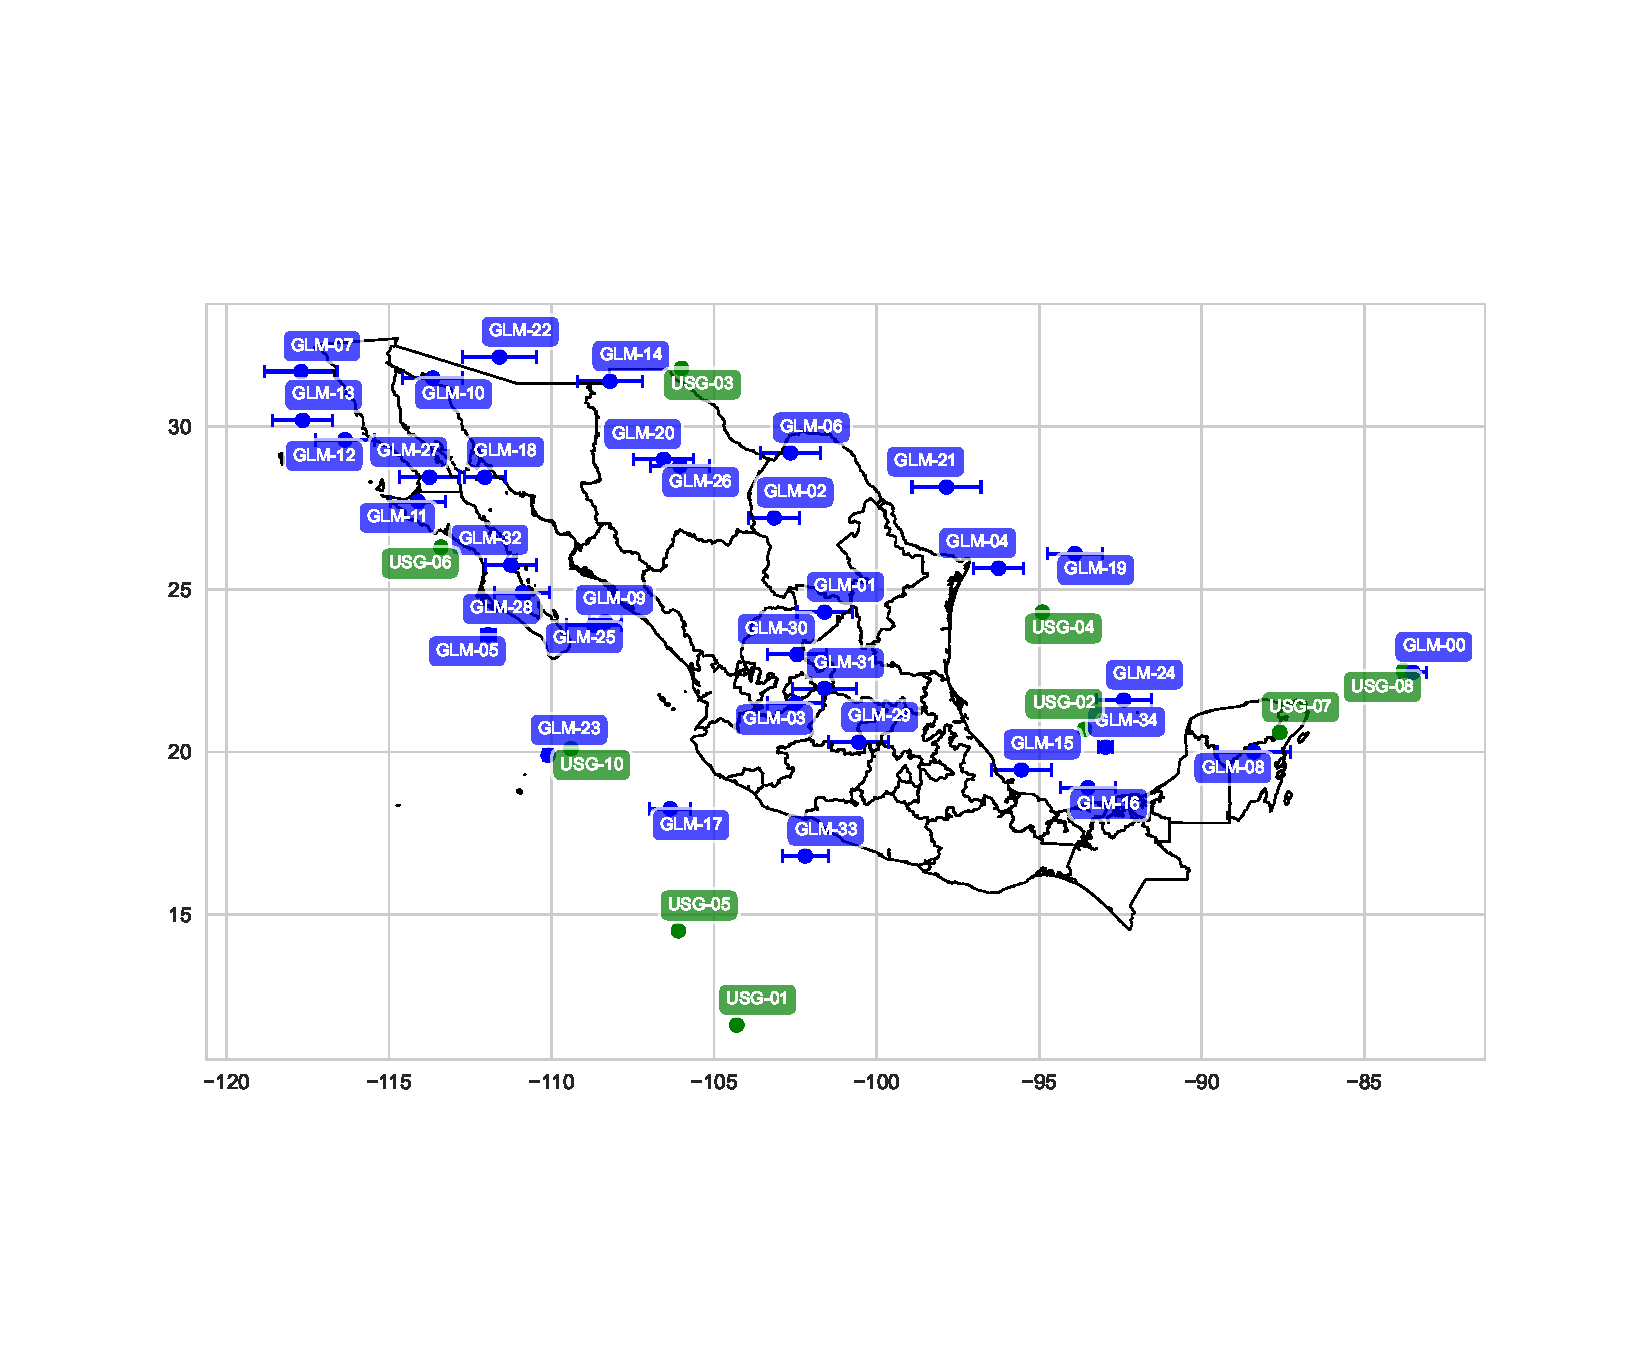
\includegraphics[width=\linewidth]{../meteors_map}
  \caption{Positions of events from table \ref{tab:table-meteors} (blue) and table \ref{tab:table-meteors-2}. The events GLM-00/USG-08 actually correpond to the same bolide, but there are little discrepancies about the position where the bolide was detecte. The same applies for the events GLM-23/USG-10 and GLM-Ven/USG-09, which not appears in the map.}
  \label{fig:meteors-map}
\end{figure}

By the other hand, we got another sample of 10 bolidesfrom US Goverment (USG) sensors from the Center for Near Earth Object Studies (CNEOS), publicly available at \url{https://cneos.jpl.nasa.gov/fireballs/}, where we may obtain directly data about bolides position, the date and time each bolide was detected, the energy released at fragmentation, the velocity and the height (the last two not availble for all bolides). As seen in table \ref{tab:table-meteors-2}, the time span is quite larger, and the released energy is generally larger. Both energy distributions are compared directly in figure \ref{fig:boxplot}. Some elements appear in both samples, since are bright enough to be detected regardless the project involved. In USG sample, the total energy of each meteor is obtained directly, but is not the case for the GLM sample. In appendix \ref{app:distance} and \ref{app:energy} we give details about how this total energy is obtained.

\begin{table*}
    \centering
  \footnotesize
  \caption{List of bolides detected in mexican territory (plus one detected near Venezuela and one detected near Cuba), detected by USG sensors.}
\label{tab:table-meteors-2}
\begin{tabular}{rrrrrrrrrrr}
       &               &                  & \multicolumn{4}{c}{Velocity (km/s)}       &                   &                 &\\\cline{4-7}
\multicolumn{1}{c}{ID}&\multicolumn{1}{c}{Date of event}&\multicolumn{1}{c}{Start Time (UT)}&\multicolumn{1}{c}{$v$}&\multicolumn{1}{c}{$v_x$}&\multicolumn{1}{c}{$v_y$}&\multicolumn{1}{c}{$v_z$}&\multicolumn{1}{c}{Latitude (deg)}&\multicolumn{1}{c}{Longitude (deg)}&\multicolumn{1}{c}{Altitude (km)} & \multicolumn{1}{c}{Energy (kT)}\\\hline
USG-01 & 1995-08-05    & 17:14:10         &      &         &           &              & 11.6              &  -104.3         &             &  0.56\\
USG-02 & 1996-07-12    & 14:04:45         &      &         &           &              & 20.7              &   -93.6         &             &  0.11\\ 
USG-03 & 1997-10-09    & 18:47:15         &      &         &           &              & 31.8              &  -106.0         &   37.0      &  0.53\\
USG-04 & 2000-01-18    & 08:33:58         &      &         &           &              & 24.3              &   -94.9         &             &  0.12\\
USG-05 & 2000-08-25    & 01:12:25         &      &         &           &              & 14.5              &  -106.1         &             &   3.1\\
USG-06 & 2005-11-15    & 05:19:07         &      &         &           &              & 26.3              &  -113.4         &   32.4      & 0.089\\
USG-07 & 2015-07-19    & 07:06:26         & 17.8 &   9.4   &  13.0     & 7.8          & 20.6              &   -87.6         &   22.0      & 0.082\\
USG-08 & 2019-02-01    & 18:17:10         & 16.3 &  -2.4   &  13.6     & 8.7          & 22.5              &   -83.8         &   23.7      &   1.4\\
USG-09 & 2019-06-22    & 21:25:48         & 14.9 & -13.4   &   6.0     & 2.5          & 14.9              &   -66.2         &   25.0      &   6.0\\
USG-10 & 2020-04-28    & 05:43:17         &      &         &           &              & 20.1              &  -109.4         &             & 0.076\\\hline  
  \end{tabular}
\end{table*}


\begin{figure}
  \centering
  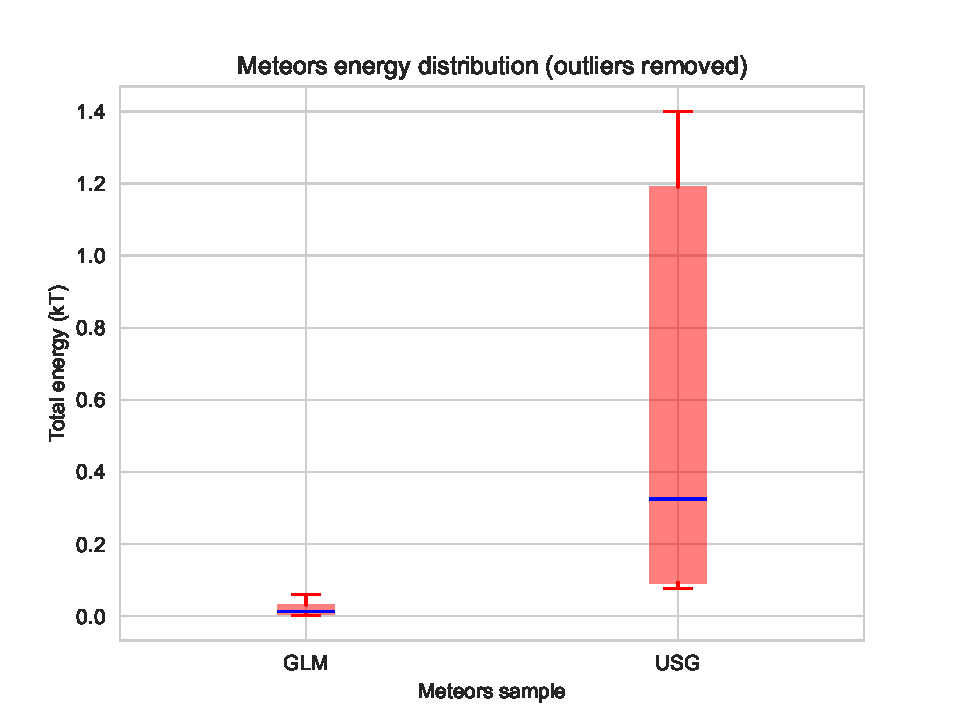
\includegraphics[width=\linewidth]{./figures/energies_boxplot}
  \caption{Comparison between released energies of bolides detected by the Geostationary Lightning Mapper and USG sensors.}
  \label{fig:boxplot}
\end{figure}


\subsection{GPS data}
\label{ssec:GPS}
%This material is based on services provided by the GAGE Facility, operated by UNAVCO, Inc., with support from the National Science Foundation and the National Aeronautics and Space Administration under NSF Cooperative Agreement EAR-1724794.

%We got RINEX data from 3 to 7 stations depending of the event location and data availability that surround the event place in all directions as possible. A list of the stations where we got RINEX data is available in table \ref{tab:table-stations}. Most of the stations lie in mexican territory, but in some cases we required data from other stations to cover events near the mexican frontier at north or south.

%\clearpage
%\onecolumn
%\footnotesize
%\begin{landscape}
%%\begin{table*}
%%    \centering
%  \begin{longtable}{llllllp{12cm}}
%      \caption{List of GPS stations used for this work.}
%      \label{tab:table-stations}
%      \endfirsthead
%      \endhead
%    \hline
%    Station name & Latitude & Longitude & \multicolumn{3}{c}{Events ID}  & Citation \\\hline
%    \multirow{4}{*}{BAR1\hyperlink{Hudnut}{${}^1$}\hyperlink{Hudnut2}{${}^5$}} & \multirow{4}{*}{33.48} & \multirow{4}{*}{-119.03} & \multirow{4}{*}{GLM-07} & \multirow{4}{*}{GLM-12} & \multirow{4}{*}{GLM-13} & UNAVCO Community, Hudnut, Kenneth, King, Nancy, Aspiotes, Aris G., Borsa, Adrian A., Determan, \\
%    &&&&&& Daniel N., Galetzka, John E., Stark, Keith F., 2005, SCIGN-PBO Nucleus GPS Network - BAR1-Santa \\
%    &&&&&& Barbara Island One P.S., The GAGE Facility operated by UNAVCO, Inc., GPS/GNSS Observations Dataset, \\
%    &&&&&& \url{https://doi.org/10.7283/T5668BHN}.\\\hline
%    \multirow{3}{*}{BLYT\hyperlink{Hudnut}{${}^1$}} & \multirow{3}{*}{33.61} & \multirow{3}{*}{-114.71} &  \multirow{3}{*}{GLM-12} & \multirow{3}{*}{GLM-13}  & & Hudnut, Kenneth, King, Nancy, Aspiotes, Aris G., Borsa, Adrian A., Determan, Daniel N., Galetzka, John \\
%    &&&&&& E., Stark, Keith F., 2006, SCIGN USGS GPS Network - BLYT-Blythe P.S., The GAGE Facility operated \\
%    &&&&&&  by UNAVCO, Inc., GPS/GNSS Observations Dataset, \url{https://doi.org/10.7283/T5HT2MKK}.\\\hline
%    \multirow{3}{*}{CN23} & \multirow{3}{*}{17.26} & \multirow{3}{*}{-88.78} &\multirow{3}{*}{GLM-08} & \multirow{3}{*}{GLM-15} & \multirow{3}{*}{GLM-16} & UNAVCO Community, 2012, COCONet GPS Network - CN23-BelmopanBZCR2012 P.S., The GAGE \\
%    &&&&&& Facility operated by UNAVCO, Inc., GPS/GNSS Observations Dataset, \\
%    &&&&&& \url{https://doi.org/10.7283/T5Q23XJH}.\\\hline
%    \multirow{3}{*}{CN25} & \multirow{3}{*}{16.23} & \multirow{3}{*}{-92.13} & \multirow{3}{*}{GLM-15} & & & UNAVCO Community, 2014, COCONet GPS Network - CN25-ComitandDMEX2012 P.S., The GAGE Facility operated by UNAVCO, Inc., GPS/GNSS Observations Dataset, \url{https://doi.org/10.7283/T57W69G7}.\\\hline
%    \multirow{3}{*}{GCFS} & \multirow{3}{*}{19.31} & \multirow{3}{*}{-81.18} & \multirow{3}{*}{GLM-08} & & & Watts, Anthony, 2016, COCONet GPS Network - GCFS-G\_CAYMAN\_CYM2014 P.S., The GAGE Facility operated by UNAVCO, Inc., GPS/GNSS Observations Dataset, \url{https://doi.org/10.7283/7ETV-X536}.\\\hline
%    \multirow{4}{*}{GMPK\hyperlink{Hudnut}{${}^1$}} & \multirow{4}{*}{33.05} & \multirow{4}{*}{-114.83} & \multirow{4}{*}{GLM-10} & & & UNAVCO Community, Hudnut, Kenneth, King, Nancy, Aspiotes, Aris G., Borsa, Adrian A., Determan, \\
%    &&&&&& Daniel N., Galetzka, John E., Stark, Keith F., 2005, SCIGN-PBO Nucleus GPS Network - GMPK-Glamis \\
%    &&&&&& Peak P.S., The GAGE Facility operated by UNAVCO, Inc., GPS/GNSS Observations Dataset, \\
%    &&&&&& \url{https://doi.org/10.7283/WCHN-H687}.\\\hline
%    \multirow{3}{*}{GUAT\hyperlink{Garnier}{${}^2$}} & \multirow{3}{*}{14.59} & \multirow{3}{*}{-90.52} & \multirow{3}{*}{GLM-16} & & & DeMets, Charles, Cosenza-Muralles, Beatriz, 2021, Central America 2018 - Guatemala, The GAGE \\
%    &&&&&& Facility operated by UNAVCO, Inc., GPS/GNSS Observations Dataset, \\
%    &&&&&& \url{https://doi.org/10.7283/KH2R-K704}.\\\hline
%\multirow{4}{*}{GUAX\hyperlink{Hudnut}{${}^1$}} & \multirow{4}{*}{28.88} & \multirow{4}{*}{-118.29} & GLM-05 & GLM-07 & GLM-11 & Hudnut, Kenneth, King, Nancy, Aspiotes, Aris G., Borsa, Adrian A., Determan, Daniel N., Galetzka, John \\
%    &&&GLM-12& GLM-13& GLM-18 & E., Stark, Keith F., 2001, SCIGN USGS GPS Network - GUAX-Isla Guadalupe P.S., The GAGE Facility \\
%    &&& GLM-25 &GLM-27 &GLM-28& operated by UNAVCO, Inc., GPS/GNSS Observations Dataset, \url{https://doi.org/10.7283/T5GX48T2}.\\
%    &&& GLM-32 &       &     &  \\\hline
%    \multirow{3}{*}{IAGX} & \multirow{3}{*}{29.03} & \multirow{3}{*}{-113.17} & \multirow{3}{*}{GLM-10} & & & Gonzalez-Ortega, Alejandro, Galetzka, John E., Gonzalez, Javier, 2018, CICESE REGNOM GPS Network \\
%    &&&&&& - IAGX-iagxREGNOMmx2018 P.S., The GAGE Facility operated by UNAVCO, Inc., GPS/GNSS  \\
%    &&&&&& Observations Dataset, \url{https://doi.org/10.7283/DGWN-A627}. \\\hline
%    \multirow{2}{*}{INEG} & \multirow{2}{*}{21.85} & \multirow{2}{*}{-102.28} & GLM-25 & GLM-26 & GLM-28  & No citations were found \\
%    &&& GLM-29 & GLM-30 & GLM-31 & \\\hline 
%    \multirow{4}{*}{KVTX} & \multirow{4}{*}{27.55} & \multirow{4}{*}{-97.89} & GLM-01 & GLM-02 & GLM-03  & UNAVCO Community, 2007, PBO GPS Network - KVTX-KingsvilleTX2006 P.S., The GAGE Facility \\
%    &&& GLM-04 & GLM-06 & GLM-19 & operated by UNAVCO, Inc., GPS/GNSS Observations Dataset, \url{https://doi.org/10.7283/T5J38QH8}.\\
%    &&& GLM-20 & GLM-21 & GLM-24 & \\
%    &&& GLM-26 &&& \\\hline
%    MDO1 & 30.68 & -104.02 & GLM-02 & & & No citations were found\\\hline
%    MGO5 & 30.68 & -104.02 & GLM-21 &GLM-26 &  & No citations were found\\\hline
%    MGW3 & 29.62 & -89.95 & GLM-19 & GLM-21 & GLM-24 & No citations were found\\\hline
%    \multirow{3}{*}{OXTH} & \multirow{3}{*}{16.29} & \multirow{3}{*}{-95.24} & \multirow{3}{*}{GLM-15} & \multirow{3}{*}{GLM-16} & & DeMets, Charles, Cabral-Cano, Enrique, 2008, Oaxaca GPS Network - OXTH-Tehuantepec P.S., The \\
%    &&&&&& GAGE Facility operated by UNAVCO, Inc., GPS/GNSS Observations Dataset, \\
%    &&&&&& \url{https://doi.org/10.7283/T5Q81B5V}.\\\hline
%    \multirow{3}{*}{OXUM\hyperlink{Graham}{${}^3$}} & \multirow{3}{*}{15.66} & \multirow{3}{*}{-96.50} & \multirow{3}{*}{GLM-34} & & & Cabral-Cano, Enrique, Salazar-Tlaczani, Luis, 2015, TLALOCNet - OXUM-oxum\_tnet\_mx2001 P.S., The \\
%    &&&&&& GAGE Facility operated by UNAVCO, Inc., GPS/GNSS Observations Dataset, \\
%    &&&&&& \url{https://doi.org/10.7283/T5J964RP}.\\\hline
%    \multirow{2}{*}{P001} & \multirow{2}{*}{31.95} & \multirow{2}{*}{-112.80} & \multirow{2}{*}{GLM-07} & \multirow{2}{*}{GLM-22} & & UNAVCO Community, 2008, PBO GPS Network - P001-Organ\_PipeAZ2007 P.S., The GAGE Facility \\
%    &&&&&& operated by UNAVCO, Inc., GPS/GNSS Observations Dataset, \url{https://doi.org/10.7283/T5DR2SGP}.\\\hline
%    \multirow{2}{*}{P014} & \multirow{2}{*}{31.97} & \multirow{2}{*}{-11.09} & GLM-10 & GLM-12 & GLM-13 & UNAVCO Community, 2008, PBO GPS Network - P014-Sahuarita\_AZ2007 P.S., The GAGE Facility \\
%    &&& GLM-14 & GLM-22 & & operated by UNAVCO, Inc., GPS/GNSS Observations Dataset, \url{https://doi.org/10.7283/T5DJ5CMK}.\\\hline
%    \multirow{2}{*}{P807} & \multirow{2}{*}{30.49} & \multirow{2}{*}{-98.82} & GLM-06 & GLM-14 & GLM-21 & UNAVCO Community, 2012, PBO GPS Network - P807-EcRockStPkTX2012 P.S., The GAGE Facility \\
%    &&& GLM-30 &&& operated by UNAVCO, Inc., GPS/GNSS Observations Dataset, \url{https://doi.org/10.7283/T5TQ5ZKM}.\\\hline
%    \multirow{2}{*}{PLPX} & \multirow{2}{*}{31.59} & \multirow{2}{*}{-115.15} & \multirow{2}{*}{GLM-10} & & & UNAVCO Community, 2011, PBO GPS Network - PLPX-Las\_PintasMX2010 P.S., The GAGE Facility \\
%    &&&&&& operated by UNAVCO, Inc., GPS/GNSS Observations Dataset, \url{https://doi.org/10.7283/T5K64G3T}.\\\hline
%    \multirow{2}{*}{PTEX} & \multirow{2}{*}{32.29} & \multirow{2}{*}{-116.52} & GLM-07 & GLM-12 & GLM-13  & UNAVCO Community, 2011, PBO GPS Network - PTEX-Testerazo\_MX2011 P.S., The GAGE Facility \\
%    &&& GLM-27 & GLM-32 & & operated by UNAVCO, Inc., GPS/GNSS Observations Dataset, \url{https://doi.org/10.7283/T5610XBP}.\\\hline 
%    \multirow{3}{*}{RG06} & \multirow{3}{*}{32.63} & \multirow{3}{*}{-107.86} & \multirow{3}{*}{GLM-22} & & & Sheehan, Anne, 2007, Rio Grande Rift GPS Network - RG06-RG06FaywodNM2006 P.S., The GAGE \\
%    &&&&&& Facility operated by UNAVCO, Inc., GPS/GNSS Observations Dataset, \\
%    &&&&&& \url{https://doi.org/10.7283/T5668BFR}.\\\hline
%    \multirow{3}{*}{RG07} & \multirow{3}{*}{32.50} & \multirow{3}{*}{-106.84} & \multirow{3}{*}{GLM-14} & & & Sheehan, Anne, 2007, Rio Grande Rift GPS Network - RG07-RG07CrucesNM2006 P.S., The GAGE  \\
%    &&&&&& Facility operated by UNAVCO, Inc., GPS/GNSS Observations Dataset, \\
%    &&&&&& \url{https://doi.org/10.7283/T5KD1W45}. \\\hline
%    \multirow{3}{*}{SG33} & \multirow{3}{*}{31.77} & \multirow{3}{*}{-106.51} & \multirow{3}{*}{GLM-06} & \multirow{3}{*}{GLM-20} & \multirow{3}{*}{GLM-26} & Harder, Steven, Kaip, Galen, Montana, Carlos, 2004, SuomiNet-G GPS Network - SG33-UTEP P.S., The \\
%    &&&&&& GAGE Facility operated by UNAVCO, Inc., GPS/GNSS Observations Dataset,  \\
%    &&&&&& \url{https://doi.org/10.7283/T50863KQ}. \\\hline
%    \multirow{3}{*}{TGMX}  & \multirow{3}{*}{20.87} & \multirow{3}{*}{-86.87} & \multirow{3}{*}{GLM-34} & & & UNAVCO Community, 2015, COCONet GPS Network - TGMX-PtoMor\_TG\_MX2015 P.S., The GAGE \\
%    &&&&&& Facility operated by UNAVCO, Inc., GPS/GNSS Observations Dataset,  \\
%    &&&&&& \url{https://doi.org/10.7283/T5154FB7}. \\\hline
%    \multirow{2}{*}{TNAM} & \multirow{2}{*}{20.54} & \multirow{2}{*}{-103.97} & GLM-17 & GLM-25 & GLM-28  & UNAVCO Community, 2014, TLALOCNet - TNAM-TNAM\_TNET\_MX2014 P.S., The GAGE Facility \\
%    &&& GLM-29 & GLM-30 & GLM-31 & operated by UNAVCO, Inc., GPS/GNSS Observations Dataset, \url{https://doi.org/10.7283/T5QF8R4R}.\\\hline
%    \multirow{2}{*}{TNAT} & \multirow{2}{*}{18.13} & \multirow{2}{*}{-98.04} & \multirow{2}{*}{GLM-15} & & & UNAVCO Community, 2014, TLALOCNet - TNAT-TNAT\_TNET\_MX2014 P.S., The GAGE Facility \\
%    &&&&&& operated by UNAVCO, Inc., GPS/GNSS Observations Dataset, \url{https://doi.org/10.7283/T5G15Z4S}. \\\hline
%    \multirow{2}{*}{TNBA} & \multirow{2}{*}{28.97} & \multirow{2}{*}{-113.55} & GLM-05 & GLM-07 & GLM-09  & UNAVCO Community, 2015, TLALOCNet - TNBA-TNBA\_TNET\_MX2014 P.S., The GAGE Facility  \\
%    &&& GLM-11 & GLM-12 & GLM-13 & operated by UNAVCO, Inc., GPS/GNSS Observations Dataset, \url{https://doi.org/10.7283/T57M0688}.\\\hline
%    \multirow{2}{*}{TNCC} & \multirow{2}{*}{18.79} & \multirow{2}{*}{-103.17} & \multirow{2}{*}{GLM-17} & & & UNAVCO Community, 2015, TLALOCNet - TNCC-TNCC\_TNET\_MX2015 P.S., The GAGE Facility \\
%    &&&&&& operated by UNAVCO, Inc., GPS/GNSS Observations Dataset, \url{https://doi.org/10.7283/T50R9MSK}.\\\hline
%    \multirow{2}{*}{TNCM} & \multirow{2}{*}{19.50} & \multirow{2}{*}{-105.04} & \multirow{2}{*}{GLM-17} & \multirow{2}{*}{GLM-23} & & UNAVCO Community, 2014, TLALOCNet - TNCM-TNCM\_TNET\_MX2014 P.S., The GAGE Facility \\
%    &&&&&& operated by UNAVCO, Inc., GPS/GNSS Observations Dataset, \url{https://doi.org/10.7283/T5B856FW}.\\\hline
%    \multirow{2}{*}{TNCN} & \multirow{2}{*}{18.55} & \multirow{2}{*}{-101.97} & \multirow{2}{*}{GLM-29} & \multirow{2}{*}{GLM-33} & & UNAVCO Community, 2016, TLALOCNet - TNCN-TNCN\_TNET\_MX2016 P.S., The GAGE Facility \\
%    &&&&&& operated by UNAVCO, Inc., GPS/GNSS Observations Dataset, \url{https://doi.org/10.7283/T5610XQM}.\\\hline
%    \multirow{4}{*}{TNCU} & \multirow{4}{*}{28.45} & \multirow{4}{*}{-106.79} & GLM-01 & GLM-02 & GLM-03  & UNAVCO Community, 2014, TLALOCNet - TNCU-CuauhtemocTN2014 P.S., The GAGE Facility \\
%    &&& GLM-06 & GLM-11 & GLM-14 & operated by UNAVCO, Inc., GPS/GNSS Observations Dataset, \url{https://doi.org/10.7283/T5V69GV2}.\\
%    &&& GLM-18 & GLM-20 & GLM-25 & \\
%    &&& GLM-26 & GLM-30 & GLM-31 & \\\hline
%    \multirow{3}{*}{TNGF} & \multirow{3}{*}{19.33} & \multirow{3}{*}{-99.18} & \multirow{3}{*}{GLM-29} & \multirow{3}{*}{GLM-33} & & Cabral-Cano, Enrique, Salazar-Tlaczani, Luis, 2016, TLALOCNet GPS Network - TNGF\_Geofisica-\\
%    &&&&&& UNAM\_Mexico\_City\_TNET\_mx2015 P.S., The GAGE Facility operated by UNAVCO, Inc., GPS/GNSS \\
%    &&&&&& Observations Dataset, \url{https://doi.org/10.7283/T53X851M}. \\\hline
%    \multirow{5}{*}{TNHM} & \multirow{5}{*}{29.08} & \multirow{5}{*}{-110.97} & GLM-05 & GLM-09 & GLM-10 & UNAVCO Community, 2014, TLALOCNet - TNHM-hermosilloTN2014 P.S., The GAGE Facility \\
%    &&& GLM-11 & GLM-12 & GLM-13 & operated by UNAVCO, Inc., GPS/GNSS Observations Dataset, \url{https://doi.org/10.7283/T5KP80FV}.\\
%    &&& GLM-18 & GLM-20 & GLM-25 & \\
%    &&& GLM-26 & GLM-27 & GLM-28 & \\
%    &&& GLM-32 &        &        & \\\hline
%    \multirow{2}{*}{TNMS} & \multirow{2}{*}{20.53} & \multirow{2}{*}{-104.80} & GLM-05 & GLM-09 & GLM-11  & UNAVCO Community, 2014, TLALOCNet - TNMS-TNMS\_TNET\_MX2014 P.S., The GAGE Facility \\
%    &&& GLM-17 & GLM-25 & & operated by UNAVCO, Inc., GPS/GNSS Observations Dataset, \url{https://doi.org/10.7283/T56H4FQ5}.\\\hline
%    \multirow{3}{*}{TNNP} & \multirow{3}{*}{16.12} & \multirow{3}{*}{-97.14} & \multirow{3}{*}{GLM-23} & & & Cabral-Cano, Enrique, Salazar-Tlaczani, Luis, DeMets, Charles, 2016, TLALOCNet - TNNP-\\
%    &&&&&& tnnp\_tnet\_mx2015 P.S., The GAGE Facility operated by UNAVCO, Inc., GPS/GNSS Observations Dataset, \\
%    &&&&&& \url{https://doi.org/10.7283/T5N29V96}. \\\hline
%    \multirow{2}{*}{TNNX} & \multirow{2}{*}{17.41} & \multirow{2}{*}{-97.22} & GLM-15 & GLM-16 & GLM-33  & UNAVCO Community, 2014, TLALOCNet - TNNX-TNNX\_TNET\_MX2014 P.S., The GAGE Facility \\
%    &&& GLM-34 &&& operated by UNAVCO, Inc., GPS/GNSS Observations Dataset, \url{https://doi.org/10.7283/T52R3PZ0}.\\\hline
%    \multirow{2}{*}{TNPP} & \multirow{2}{*}{31.34} & \multirow{2}{*}{-113.63} & GLM-07 & GLM-10 & GLM-18 & UNAVCO Community, 2015, TLALOCNet - TNPP-TNPP\_TNET\_MX2015 P.S., The GAGE Facility \\
%    &&& GLM-22 &&& operated by UNAVCO, Inc., GPS/GNSS Observations Dataset, \url{https://doi.org/10.7283/T5CC0Z0M}.\\\hline
%    \multirow{2}{*}{TNSJ} & \multirow{2}{*}{16.17} & \multirow{2}{*}{-96.49} & \multirow{2}{*}{GLM-33} & & & UNAVCO Community, 2016, TLALOCNet - TNSJ-tnsj\_tnet\_mx2015 P.S., The GAGE Facility operated by \\
%    &&&&&& UNAVCO, Inc., GPS/GNSS Observations Dataset, \url{https://doi.org/10.7283/T59S1PF1}.\\\hline
%    \multirow{3}{*}{TSFX} & \multirow{3}{*}{30.93} & \multirow{3}{*}{-114.81} & \multirow{3}{*}{GLM-07} & \multirow{3}{*}{GLM-27} & \multirow{3}{*}{GLM-32} & Gonzalez-Ortega, Alejandro, Galetzka, John E., Gonzalez, Javier, 2018, CICESE REGNOM GPS Network \\
%    &&&&&& - TSFX-tsfxREGNOMmx2016 P.S., The GAGE Facility operated by UNAVCO, Inc., GPS/GNSS \\
%    &&&&&& Observations Dataset, \url{https://doi.org/10.7283/AGEA-2G27}.\\\hline
%    \multirow{3}{*}{UAGU} & \multirow{3}{*}{21.92} & \multirow{3}{*}{-102.32} & GLM-01 & GLM-02 & GLM-03  & Cabral-Cano, Enrique, Salazar-Tlaczani, Luis, 2015, TLALOCNet - UAGU-uagu\_tnet\_mx2008 P.S., The \\
%    &&& GLM-04 & GLM-06 & GLM-09 & GAGE Facility operated by UNAVCO, Inc., GPS/GNSS Observations Dataset, \\
%    &&& GLM-11 & GLM-20 &        & \url{https://doi.org/10.7283/T5513WK7}.\\\hline
%    \multirow{3}{*}{UCOE\hyperlink{Graham}{${}^3$}} & \multirow{3}{*}{19.81} & \multirow{3}{*}{-101.69} & GLM-03 & GLM-06 & GLM-30 & Cabral-Cano, Enrique, Salazar-Tlaczani, Luis, 2015, TLALOCNet - UCOE-ucoe\_tnet\_mx2003 P.S., The \\
%    &&& GLM-31 &&& GAGE Facility operated by UNAVCO, Inc., GPS/GNSS Observations Dataset, \\
%    &&&&&& \url{https://doi.org/10.7283/T51834VW}. \\\hline
%    \multirow{3}{*}{UGEO\hyperlink{Marquez}{${}^4$}} & \multirow{3}{*}{20.69} & \multirow{3}{*}{-103.35} & \multirow{3}{*}{GLM-03} & & & Marquez-Azua, Bertha, DeMets, Charles, Cabral-Cano, Enrique, Salazar-Tlaczani, Luis, 2015, \\
%    &&&&&& TLALOCNet - UGEO-ugeo\_tnet\_mx1998 P.S., The GAGE Facility operated by UNAVCO, Inc., GPS/GNSS \\
%    &&&&&& Observations Dataset, \url{https://doi.org/10.7283/T58S4N9N}. \\\hline
%    \multirow{2}{*}{UHSL} & \multirow{2}{*}{29.57} & \multirow{2}{*}{-95.65} & \multirow{2}{*}{GLM-19} & & & Wang, Guoquan, 2014, HoustonNet GPS Network - UHSL-SugarLandUSA2014 P.S., The GAGE Facility \\
%    &&&&&& operated by UNAVCO, Inc., GPS/GNSS Observations Dataset, \url{https://doi.org/10.7283/T55X271S}.\\\hline
%    \multirow{3}{*}{UHWL} & \multirow{3}{*}{30.06} & \multirow{3}{*}{-94.98} & \multirow{3}{*}{GLM-31} & & & Wang, Guoquan, 2014, HoustonNet GPS Network - UHWL-West Liberty Airport(Deep) P.S., The GAGE \\
%    &&&&&& Facility operated by UNAVCO, Inc., GPS/GNSS Observations Dataset,  \\
%    &&&&&& \url{https://doi.org/10.7283/T53R0R5P}. \\\hline
%    \multirow{3}{*}{UNPM} & \multirow{3}{*}{20.86} & \multirow{3}{*}{-86.86} & GLM-08 & GLM-15 & GLM-16  & UNAVCO Community, 2012, COCONet GPS Network - UNPM-Puerto\_Morelos\_MX\_2007 P.S., The \\
%    &&& GLM-24 &&& GAGE Facility operated by UNAVCO, Inc., GPS/GNSS Observations Dataset, \\
%    &&&&&& \url{https://doi.org/10.7283/J1GD-5S40}.\\\hline
%    \multirow{3}{*}{USMX} & \multirow{3}{*}{29.82} & \multirow{3}{*}{-109.68} & GLM-12 & GLM-13 & GLM-14  & Bennett, Rick, 2004, Northwest Mexico GPS Network - USMX-Universidad de la Sierra P.S., The GAGE \\
%    &&& GLM-22 & GLM-26 & GLM-28 & Facility operated by UNAVCO, Inc., GPS/GNSS Observations Dataset, \\
%    &&&&&& \url{https://doi.org/10.7283/T5W957CQ}.\\\hline
%    \multirow{3}{*}{UXAL\hyperlink{Graham}{${}^3$}} & \multirow{3}{*}{19.52} & \multirow{3}{*}{-96.92} & GLM-04 & GLM-15 & GLM-16  & Cabral-Cano, Enrique, Salazar-Tlaczani, Luis, 2015, TLALOCNet - UXAL-uxal\_tnet\_mx2005 P.S., The \\
%    &&& GLM-19 & GLM-24 & GLM-31 & GAGE Facility operated by UNAVCO, Inc., GPS/GNSS Observations Dataset, \\
%    &&& GLM-34 &        &        & \url{https://doi.org/10.7283/T5DJ5D1C}.\\\hline
%    \multirow{2}{*}{WEPD} & \multirow{2}{*}{29.69} & \multirow{2}{*}{-95.23} & \multirow{2}{*}{GLM-21} & & & Wang, Guoquan, 2014, HoustonNet GPS Network - WEPD-willmselementary P.S., The GAGE Facility \\
%    &&&&&& operated by UNAVCO, Inc., GPS/GNSS Observations Dataset, \url{https://doi.org/10.7283/T5NZ85RB}. \\\hline
%    \multirow{2}{*}{WMOK} & \multirow{2}{*}{34.74} & \multirow{2}{*}{-98.78} & \multirow{2}{*}{GLM-21} & & & UNAVCO Community, 2005, PBO GPS Network - WMOK-WichitaMtnOK2005 P.S., The GAGE Facility \\
%    &&&&&& operated by UNAVCO, Inc., GPS/GNSS Observations Dataset, \url{https://doi.org/10.7283/T59021Q6}. \\\hline
%    \multirow{4}{*}{WWMT\hyperlink{Hudnut}{${}^1$}} & \multirow{4}{*}{33.96} & \multirow{4}{*}{-116.65} & \multirow{4}{*}{GLM-07} & \multirow{4}{*}{GLM-12} & \multirow{4}{*}{GLM-13} & Hudnut, Kenneth, King, Nancy, Aspiotes, Aris G., Borsa, Adrian A., Determan, Daniel N., Galetzka, John \\
%    &&&&&& E., Stark, Keith F., 2006, SCIGN USGS GPS Network - WWMT-Whitewater Mountain P.S., The GAGE \\
%    &&&&&& Facility operated by UNAVCO, Inc., GPS/GNSS Observations Dataset,  \\
%    &&&&&& \url{https://doi.org/10.7283/T5H993F2}. \\\hline
%    \multirow{2}{*}{YESX} & \multirow{2}{*}{28.38} & \multirow{2}{*}{-108.92} & GLM-09 & GLM-11 & GLM-14  & Bennett, Rick, 2004, Northwest Mexico GPS Network - YESX-Yecora P.S., The GAGE Facility operated \\
%    &&&GLM-20 & GLM-23 & GLM-25 & by UNAVCO, Inc., GPS/GNSS Observations Dataset, \url{https://doi.org/10.7283/T5RJ4GPF}.\\\hline
%    
%%    % \end{table*}
%  \end{longtable}
%    \begin{minipage}{0.9\linewidth}
%      \footnotesize
%      Related articles:
%      
%      \hypertarget{Hudnut}{${}^1$}\citet{Hudnut:2002},
%      %
%      \hypertarget{Garnier}{${}^2$}\citet{Garnier:2021}, 
%      %
%      \hypertarget{Graham}{${}^3$}\citet{Graham:2016}
%      
%      \hypertarget{Marquez}{${}^4$}\href{https://doi.org/10.7283/T58S4N9N}{B. Marquez-Azua, E. Cabral-Cano, F. Correa-Mora and C. DeMets, 2004. A model for Mexican neotectonics based on Nationwide GPS measurements, 1993-2001, Geofisica Internacional, v. 43, p.319-330}
%      
%      \hypertarget{Hudnut2}{${}^5$}\href{https://doi.org/10.7283/T5668BHN}{Hudnut, K. W., Y. Bock, J. E. Galetzka, F. H. Webb, and W. H. Young, The Southern California Integrated GPS Network (SCIGN), Proceedings of the International Workshop on Seismotectonics at the Subduction Zone, Y. Fujinawa (ed.), NIED, Tsukuba, Japan, pp. 175-196, 1999}    
%    \end{minipage}
%  \end{landscape}
%  \clearpage
%  \twocolumn

%  The obtained RINEX files are compressed in Hatanaka format, developed at the Geographical Survey Institute by Y. Hatanaka \citep{Kumar:2012}. From this files we may estimate the Slant Total Electron Content (sTEC) and the Vertical Total Electron Content (vTEC) which may be computed in the following way:

  The Total Electron content along the integrated path of the link $(s_i)$ at the frequency $f_i$ can be inferred from the phase delay $L_i$ of the frequency $f_i$ \citep{Emery:2017}:
  \begin{align}
    L_i = s_i - \frac{\SI{40.3082}{m^3.s^{-1}}}{f_i^2}sTEC_i
  \end{align}
  Combining two observations at two different frequencies $f_1$ and $f_2$ we may obtain two different phase delays $L_1$ and $L_2$ and derive the TEC along the signal path:

  \begin{align}
    sTEC = \frac{f_1^2f_2^2\left(L_1-L_2\right)}{\SI{40.3082}{m^3.s^{-1}}\left(f_1^2-f_2^2\right)}
  \end{align}

  In the other hand, the Vertical Total Electron Content (vTEC) is computed from the sTEC as follows \citep{Kumar:2012}:
  \begin{align}
    vTEC = \frac{sTEC-\left[b_R+b_S\right]}{S(\theta_I)}
  \end{align}

  where $b_R$ and $b_S$ are receiver and satellite biases, respectively. $\theta_I$ is the elevation angle in degrees, $S(\theta_I)$ is the obliquity factor with zenith angle $\psi$ at the Ionospheric Pierce Point (IPP):

  \begin{align}
    S(\theta_i) = \frac{1}{\cos\psi} = \left\lbrace 1-\frac{R_E\cos\theta_I}{R_E+h}\right\rbrace^{-1/2}
  \end{align}

  Where $R_E$ is the Earth radius in km and $h=\SI{350}{km}$ is the ionospheric shell above the earth's surface.

  Both parameters sTEC and vTEC are computed using a software developed by Gopi K. Seemala, publicly available at \url{https://seemala.blogspot.com/}.

  
%For the selected sample, we obtained RINEX data from the TlalocNet \citep{Cabral-Cano:2018} and UNAVCO network databases to study potential alterations in the ionospehre due to the presence of the passing meteor at the day the meteor was reported. For each event, we downloaded data from stations that surrounds the place where the event was detected (usually 3 to 5 stations. )The list of the sample meteors is shown in table \ref{tab:table-meteors}. The events are in chronological order. The reported duration, latitude and longitude correspond to the mean between measurements from satellites GOES-16 and GOES 17; in the same way, the uncertainties correspond to the standard deviation. Also their respective positions are available in figure \ref{fig:meteors-map}, where each label correspond to the ID (first column) of table \ref{tab:table-meteors}.
     
%Using the data provided by TlalocNet and UNAVCO, we procceeded to obtain TEC parameters with the GPS\_GOPI software, available at \url{https://seemala.blogspot.com/}. This software takes as input the RINEX data (the navigation file is no strictly neccesary), and the outuput consists in in the vTEC and sTEC measurements for the PRNs of the whole day the event occurred, as well as the averaged TEC as function of time. We obtained vTEC maps for the events in table (\ref{tab:table-meteors}) and their respective next and previous day.
     
%Final idea: use GOPI software to get the vTEC data from the day of each event and the previous days.


\section{Bolides physical parameters}
\label{sec:bolides}
\begin{table}
    \centering
     \caption{Caribbean meteor possible physical properties obtained with  algorithm  , assuming a density of \SI{3000}{kg.m^{-3}}}
    \begin{tabular}{lr}\toprule
       Initial Velocity  &  \SI{19.9}{km.s^{-1}}\\
        Initial mass & \SI{340}{kg} \\
        Entry angle (deg) & 64 \\
        \bottomrule
    \end{tabular}
    \label{tab:meteor-properties}
\end{table}

Using the estimation of the meteor energy and velocity from table \ref{tab:Meteor-parameters}, the trajectory angle estimated in appendix \ref{app:velocity} from the velocity components of $64.4^\circ$ and assuming the meteor has a density of \SI{3000}{kg.m^-3}, consistent with the composition of \textit{condrites} (we must assure or edit this last statement), we estimated the initial velocity, initial mass and entry angle using (add citation and more text and once got the references) ...%we are capable to estimate other bolides parameters, such as the mass. For that we used a Fragment Cloud Model \citep{Wheeler:2017}. To obtain the bolide mass, we must have previous knowledge of its velocity. Based on the few events of the USG sample where we could extract the velocity (see table \ref{tab:table-meteors-2}), we tried three models of bolides mass as a function of its releasing energy: the low velocity model, which assumes a velocity of $\sim \SI{15}{km.s{^-1}}$, medium velocty $v \sim \SI{16}{km.s{^-1}}$ and high velocity $v \sim \SI{18}{km.s{^-1}}$. The resultant masses can be seen in figure \ref{fig:energy-mass}. For the rest of the sample we need to assume that the bolides velocity is within this range or close enough in order to get a reasonable estimation of its mass.
\section{Ionospheric background and vTEC maps}
\label{sec:vTEC-maps}
     
In progress ...
%Ionospheric perturbations also can take place due to space weather and geomagnetic storms. So, in order to discard such events we investigated the space weather in the day each event occured. In figure (name) we present the geomagnetic \textit{Kp} index for some events. We discarded events whose Kp index is equal or grater than 4 in the day of the event or shortly before. Also we present in figure (name) the vTEC perturbation maps for the same events in a three day series, centered in the event date. The estimated meteor trajectory, obtained from the GLM data is presented in black, continous line, while the linear fit to the GOES-16 and GOES-17 data are presented with the red dashed line, and work as boudary errors.
     
     
     
%\section{Frecuency Analysis}
     
\section{Discussion}
\label{sec:discission}

We collected data for a sample of meteors which were detected around Mexican territory, or with some exceptions, meteoroids that released enough energy to have a good chance to get a vTEC disturbance with nearby GPS stations. We used data from the GLM, where the total energy was estimated from light curves, and USG sensors, where energy data is available. We used the few events which are present in both samples to re-calibrate the energy obtained for the GLM sample since in this few cases the energy estimated with the GLM data is systematically lower than the energy reported by USG sensors. Using the resulting energies, we estimated the bolides mass using a Fragment Cloud Model assuming a certain velocity range. 

We have collected GPS data of nearby stations where the event was detected at the date each event occured, and one day before as comparison. We obtained the the vTEC series and we detrended them to remove the effects of Earth rotation and solar activity and make the wave-like features more evident. With these data, we used a wavelet transform using a Morlet wavelet to discover the frequencies at which vTEC perturbations may be produced, how intense these perturbations are and the time interval of these perturbations. If two different stations detect perturbations at the same frequencies that means that a vTEC perturbation was detected with such stations. We have observed that the distribution of wavelet coherent signal show us that the propagation of ionospheric disturbances have a time intervals of occurrence of a two hours from the spectrograms. 

%\section{How to include a figure?}
%Change the file name of the figure below with your own 
%figure. And remember to change the figure caption too!
%\begin{verbatim}
%\begin{figure}
%  \centering
%  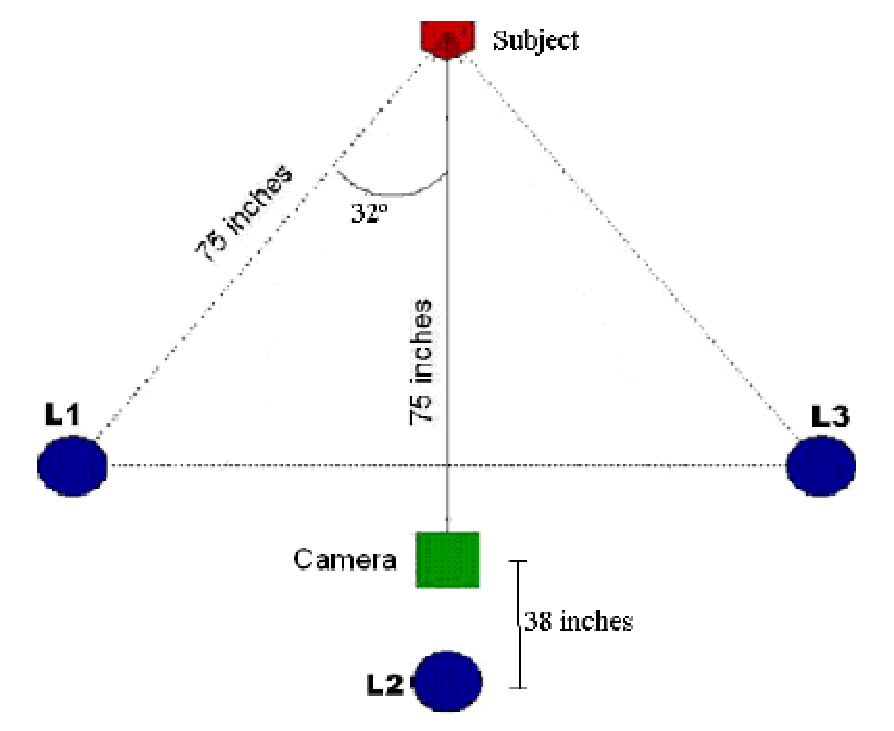
\includegraphics[scale=0.5]{fig01}
%  \caption{Write the figure caption here.}
%  \label{fig:pendulum}
%\end{figure}
%\end{verbatim}
%\begin{figure}
%\centering
%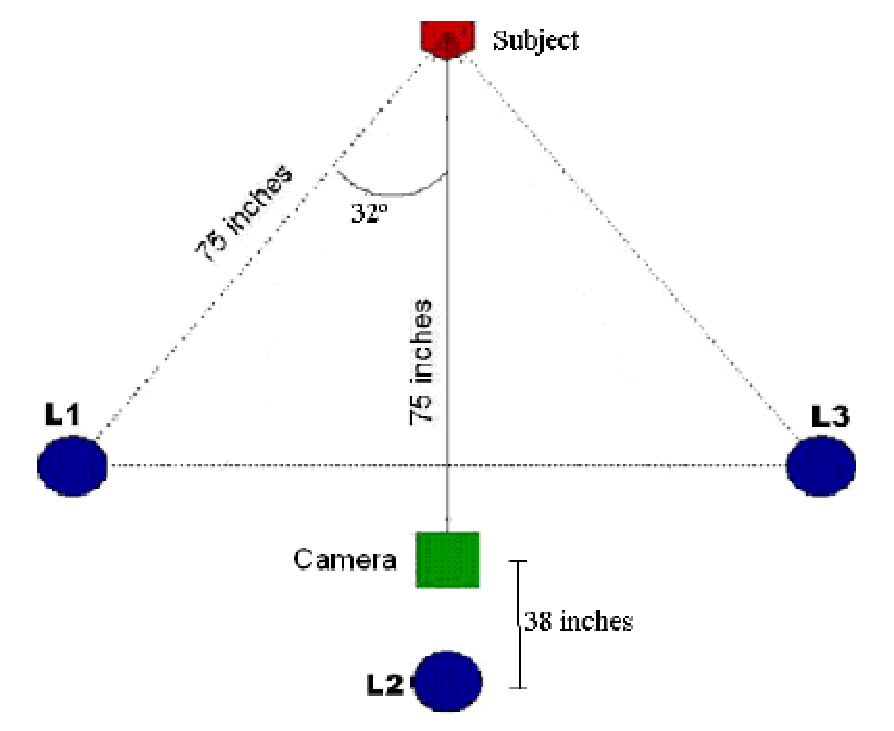
\includegraphics[scale=0.5]{fig01.pdf}
%\caption{Write the figure caption here.}
%\label{fig:pendulum}
%\end{figure}

%\subsection{And a table?}
%Just replace the text/values in the template table below 
%with your own. You can change the number of 
%lines/rows as necessary.
   
%\begin{table*}
%\centering
%\caption{Title of the table should be at the top}
%\begin{tabular}{|l|l|l|l|}
%\hline
%Column Name1    & Column Name2 & Column Name3 & Column Name4 \\
%\hline
%Parameter Name1 & Value        & Value        & Value        \\
%\hline
%Parameter Name2 & Value        & Value        & Value        \\
%\hline
%Parameter Name3 & Value        & Value        & Value        \\
%\hline
%\end{tabular}
%\end{table*}

%\subsection{Equations}
%Conventionally, in mathematical equations, variables and
%anything that represents a value appear in italics. 
%All equations should be numbered for easy referencing. 
%The number should appear at the right margin.
%\begin{eqnarray}
%S'_{\mathrm{pg}} = \frac{S_{\mathrm{pg}} - \mathrm{min}(S_{\mathrm{pG}})}
%  {\mathrm{max}(S_{\mathrm{pG}} - \mathrm{min}(S_{\mathrm{pG}}))}
%\end{eqnarray}
%In mathematical expressions 
%in running text "/" should be used
%for division (not a horizontal line).

%\section{Citations}
%Citations in the text can be made using\\[6pt]
%\verb+\citet{NewmanGirvan2004}+\\[6pt]
%for citation in running text like in 
%\citet{NewmanGirvan2004} or using\\[6pt]
%\verb+\citep{Vehlowetal2013,NewmanGirvan2004}+\\[6pt]
%for citation within parentheses like in 
%\citep{Vehlowetal2013,NewmanGirvan2004}.

%Please use the actual \verb+\cite+ command in the text.
%Also, please double-check the \verb+\citep+ command.

%\section{Reference style}
%You can include the references in the main text file in \LaTeX
%format. Alternately, you can include a separate bibliography
%file (refs.bib in this example) and run the following set of 
%commands:
%\begin{verbatim}
%==================

%pdflatex myfile.tex

%bibtex myfile (no extension in this line!)

%pdflatex myfile.tex

%pdflatex myfile.tex

%==================
%\end{verbatim}

%\section{A sample entry in the bibliography file}
%{\fontsize{7.5pt}{9.6pt}\selectfont
%\begin{verbatim}
%==================

%@ARTICLE{NewmanGirvan2004,
%  author  = {Newman, M. E. J. and Girvan, M.},
%  title   = {Finding and evaluating community 
%               structure in networks},
%  journal = {Phys. Rev. E.},
%  volume  = {69},
%  number  = {21},
%  year    = {2004},
%  pages   = {026113}
%}

%==================
%\end{verbatim}
%}

\section{Acknowledgments}
\label{sec:acknowledgments}
\input{../Acknowledgments}
%% Bibliography
%% Author year style
\appendix
% \appendixpage
% \addappheadtotoc

% This is tha appendix, where we may insert detailed mathematical proccedures or other data which may be useful but also will make the main
% text too large so this should be consulted only in case of neccesity

\section{Estimation of distances to meteors}
\label{app:distance}
The distance between the GOES satellite and the meteor, neccesary to estimate the radiated energy is calculated as follows:

\begin{align}
  R = \left|\vec{r}_{GLM} - \vec{r}_{obj} \right|
\end{align}

where $\vec{r}_{GLM}$ is the vector position of the GLM satellite and $\vec{r}_{obj}$ is the vector position of the meteor.

In cartesian coordinates, the distance $R$ is given by:

\begin{align}
  R &= \left((x_{GLM}-x_{obj})^2 + (y_{GLM}-y_{obj})^2 + (z_{GLM}-z_{obj})^2\right)^{1/2} \label{eq:R}\\
\end{align}

The transformation to spherical coordinates is given by:

\begin{align}
  x = r\cos\phi\cos\theta \label{eq:xtoR}\\
  y = r\sin\phi\cos\theta \label{eq:ytoR}\\
  z = r\sin\theta \label{eq:ztoR}
\end{align}

Where $r$ is measured from the center of the earth, $ -180^\circ < phi <= 180^\circ$ represents the longitude; is positive at east of Greenwich meridian, and negative eastwards. $\-90^\circ <= \theta <= 90^\circ$ represents the latitude and is positive at the north of equator and negative southwards.

Substituting the transform (\ref{eq:xtoR} - \ref{eq:ztoR}) into (\ref{eq:R}), using elemental trigonometry and considering both GLM satellites lie into the equator ($\theta_{GLM}=0$) we get:

\begin{align}
  R^2 &= r_{GLM}^2 + r_{obj}^2 - 2r_{GLM}r_{obj}f(\theta_{obj}, \phi_{obj}, \phi_{GLM}) \label{eq:R2}\\
  \mathrm{where:} & f(\theta_{obj}, \phi_{obj}, \phi_{GLM}) = \cos\theta_{obj}\cos\left(\phi_{GLM}-\phi_{obj}\right)
\end{align}

Since $r_{GLM}$ and $r_{obj}$ are measured from the center of the arth ge find that:

\begin{align}
  r_{GLM} &= r_{earth} + h_{GLM} \label{eq:rg}\\
  r_{obj} &= r_{earth} + h_{obj} \label{eq:ro}
\end{align}

Substituting (\ref{eq:rg}, \ref{eq:ro}) into \ref{eq:R2} and considering that $h_{obj} \ll h_{GLM}$ we get:

\begin{align}
  \begin{split}
    R^2 = 2r_{earth}^2\left(1-f(\theta_{obj}, \phi_{obj}, \phi_{GLM})\right) +2r_{earth}h_{GLM}\\
    \left(1-f(\theta_{obj}, \phi_{obj}, \phi_{GLM})\right) + h_{GLM}^2 - 2h_{GLM}h_{obj}f(\theta_{obj}, \phi_{obj}, \phi_{GLM})
    \end{split}
\end{align}

\section{Energy estimation}
\label{app:energy}
The total radiant energy emmited is calculated integrating over all the time and all directions. The first is obtained simply summing all the light curve points. In the other hand, to integrate over all directions, we multiply the GLM event energies by the factor (\SI{1.695e18}{})(\SI{1.018e3}{})$\left(\frac{R}{35780~km}\right)^2$ \citep{Jenniskens:2018}. This factor also considers that the GLM only detects light from the OI line. Then, we obtain the luminous efficiency $\tau_1$ (i.e the fraction of the total energy converted into radiation) following \citet{Brown:2002}:
\begin{align}
  \tau_1 = (0.1212\pm 0.0043)E_0^{0.115\pm 0.075}
\end{align}

Where $E_0$ is the luminous energy calculated from integrating GLM reported energies (in kilotons). Finally the total estimated energy is $E = E_0/\tau_1$. We may compare the resulting GLM energies with the energies reported by USG sensors using the events which belong to both samples, and we noticed that the energies obtained with GLM data is systematically lower than the energies reported by the USG sensors. In this work we assumed that this discrepancy is due to the GLM sensors does not detect the full meteor paths, just a fraction of the total radiated energy. To solve this problem we made a linear fit between the derived energies and the energies reported in the USG sample for the events which appear in both samples, and recallibrate the energies of the rest of the GLM sample. The linear fit is shown in figure \ref{fig:lin_fit}. We used the linear fit slope as the recallibration factor and the residuals as the error, we neglected the y-intercept term because this term is much larger than the most energies in the GLM sample and strongly affects the recallibrated energy.

\begin{figure}
  \centering
  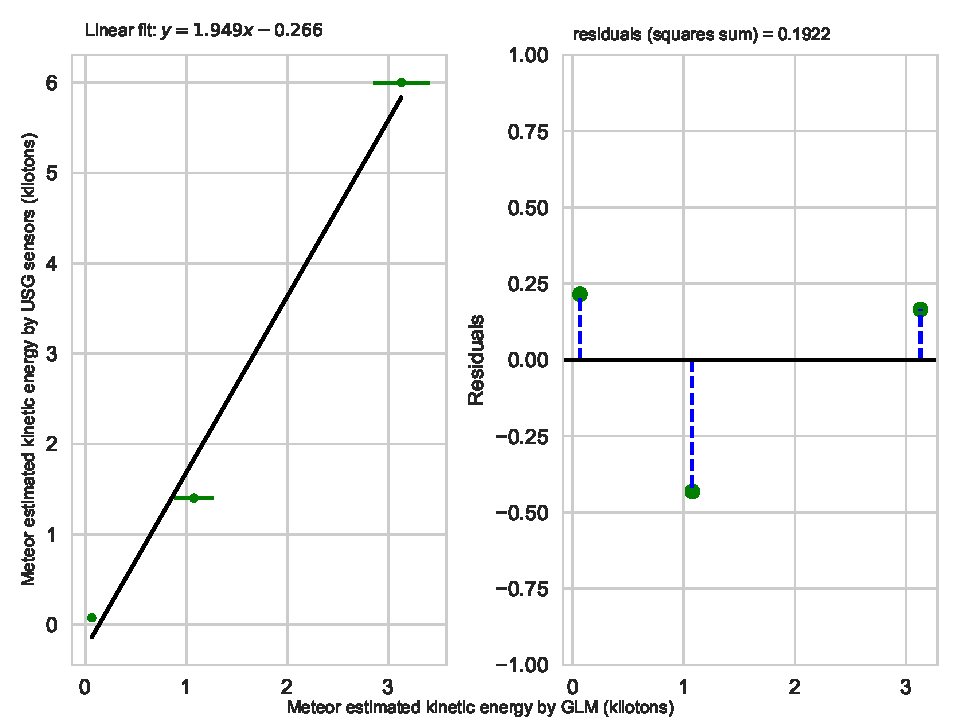
\includegraphics[width=\linewidth]{../energy_fit}
  \caption{Left: Linear fit between energies calculated from GLM data and energies reported by USG sensors. Right: Residuals of the fit, used as error in the recallibration factor. The three events used for this linear fit are GLM-00 (the cuban meteoroid), GLM-23 and GLM-Ven (Venezolan meteoroid).}
  \label{fig:lin_fit}
\end{figure}



\bibliographystyle{model5-names}
\biboptions{authoryear}
\bibliography{../bibliography}

\end{document}

%%

